\pdfoutput=1

\documentclass{l4proj}

%
% put any packages here
%
\usepackage{subcaption}
\usepackage{enumitem}
\usepackage{url}
\usepackage{booktabs}
\usepackage{alltt}
\usepackage{wrapfig}

\begin{document}
\title{Animation of the Contextual Analysis and Code Generation Phases of a Compiler}
\author{David Robertson}
\date{January 1, 2000}
\maketitle

\begin{abstract}

\end{abstract}

\educationalconsent
%
%NOTE: if you include the educationalconsent (above) and your project is graded an A then
%      it may be entered in the CS Hall of Fame
%
\tableofcontents
%==============================================================================

\chapter{Introduction}
\pagenumbering{arabic}
With increasing technological advances and furthering levels of software abstraction, some may consider compilation to be a slightly esoteric subject, in that, broad knowledge of compilation theory is unnecessary in a modern environment and required only in a small number of highly specialised industries. Yet, remaining as a cornerstone of a computer science curriculum at many schools and universities is the art of compiler construction, behaviour and optimisation. Why is this?

When questioned on the necessity of teaching compilation, Niklaus Wirth, the creator of the \textit{Pascal} programming language and renowned lecturer of compiler design states, ``\textit{knowledge about system surfaces alone is insufficient in computer science; what is needed is an understanding of contents}'' \cite{WirthTheory}. Wirth's view is one that many share, in the respect that the most successful computer scientists must have more than a superficial understanding of which approaches to follow in a given situation. They must understand how various components interact and why they behave the way they do. To gain a true understanding of the building blocks of computer science is to gain a greater insight into the scientific and mathematical concepts within the field, which provides the most effective means of making informed technological decisions. 

Compilation theory is a foundational notion of computer science, upon which a larger syllabus can be developed. To students, the benefits of learning about compilation are perhaps not in its direct application, but in its ability to act as the stepping stone that facilitates a more comprehensive grasp of other concepts; concepts which themselves are grounded in compilation theory.  

\section{Motivation}
Compilation can often be a challenging field to teach effectively. Many components of compilation involve the generation and traversal of complex, abstract data structures. Abstract, conceptual notions such as these are notoriously difficult both for students to understand and for educators to demonstrate. We desire to find a solution to this problem by creating techniques that provide concrete representations of abstract ideas.

In response to this issue, a common approach employed by educators is to attempt to visualise the data structures and the traversals over them. The educator usually does this by creating some sort of ``slideshow'', using an application such as Microsoft PowerPoint. The slides contain a pictorial representation of the data structure in question, and each slide demonstrates a distinct step of the traversal over that data structure. For example, an educator seeking to teach students about a depth-first traversal over a binary tree might design their slideshow similarly to Figure \ref{fig:slideshow}. In Figure \ref{fig:slideshow} we see that each consecutive slide illustrates the next step of the traversal by highlighting the corresponding node.

\begin{figure}
\centering
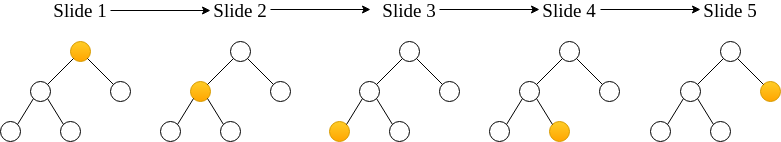
\includegraphics[scale=0.5]{images/slideshow.png}
\caption{A sequence of slides demonstrating a depth-first traversal over a binary tree}
\label{fig:slideshow}	
\end{figure}

Whilst using a slideshow to demonstrate these concepts does provide part of the solution to representing abstract notions, they have several limitations. Firstly, to create visualisations in this way is an arduous task on behalf of the educator, realistically meaning that the demonstration must remain short. Secondly, there is a limited amount of control over the “playback” of the slides in regards to playing, pausing, rewinding and restarting; which of these functions is available depends on the choice and availability of slideshow application. Thirdly, and most importantly, the educator is restricted to showing pre-determined examples only. In the case of compilation, there is effectively an infinite number of ways the compilation process may occur depending on the input to the compiler. This means pre-determined examples are almost guaranteed to omit certain details, making it difficult for students to achieve a broad and complete understanding.

\section{Aims}
This project aims to alleviate or solve many of the issues currently faced in attempts to create effective visualisations of various compilation concepts. The project will provide a web application in which users will be able to animate the \textit{\textbf{contextual analysis}} and \textit{\textbf{code generation}} phases of the \textit{\textbf{Fun}} compiler. The animation will incorporate a representation of an \textit{\textbf{abstract syntax tree}} (AST). 

Contextual analysis and code generation are two different stages of compilation which aim to validate certain aspects of the compiler's input and construct some appropriate output. The behaviour of these stages is expressed by traversals over an AST. An AST is a tree-based data structure that represents the hierarchical syntactic structure of a section of code. Fun is a simple, educational programming language equipped with a compiler. Chapter 3 introduces all of these concepts in considerably more detail. 

The application will allow users to supply programs written in the Fun language as input to the Fun compiler. The user can then choose to animate either the contextual analysis or code generation phase of the resulting compilation. In order to demonstrate how the compiler traverses the AST during these phases, nodes within the tree will be highlighted consecutively corresponding to the progression of the traversal, similar to the method displayed in Figure \ref{fig:slideshow}. In general, the application should:
\begin{itemize}
\item Allow a user to input any syntactically valid program written in the Fun language.
\item Animate the contextual analysis phase of a program's compilation. 
\item Animate the code generation phase of a program's compilation.
\item Augment the animation with explanatory messages that provide insight into the internal logic of the compiler.
\item Augment the animation with any other relevant supplementary information.
\item Allow the animation to be played, paused or stepped through (backwards and forwards).
\end{itemize}

The application, which will act as an educational tool, resolves many of the problems we previously discussed with respect to slideshow-based visualisations. Most obviously, educators are no longer required to create the visualisations themselves, a time consuming process. They can simply project footage of the application to students within a classroom setting, or even better, direct students to access the application themselves. The application aims to implement playing, pausing, rewinding and restarting of the animation, meaning the previous issues of playback limitations are removed as long as the user has access to a web browser. The application also allows any arbitrary Fun program to be animated, meaning the restriction of only showing examples with a pre-determined input is eliminated. Additionally, the application desires to supply in-depth automated analytical details (in the form of explanatory messages and supplementary information), something that is not currently possible by present techniques. The application will hopefully provide a better means for those looking to learn but also remove some of the struggle taken on by educators in teaching the topic.

\section{Outline}
The rest of this report is organised as follows: Chapter 2...

\chapter{Background \& Related Work}
Despite the animation of compilers being a considerably novel area of research and development, attempts to visualise computing algorithms date as far back as the 1980s \cite{BentleyKernighan}. The vast majority of work in the field up to now has been focused on the animation of complex, yet small and well-defined algorithms, most notably sorting algorithms or tree traversals.

Indeed, compilation is certainly not small nor particularly well-defined (in that the behaviour of the compiler can vary significantly depending on the implementation), however, many aspects of typical algorithm animations (such as tree traversals) can be found in abundance within a potential compiler animation. Ultimately, compilation itself is just an algorithm,  and it would seem logical to assume that any lessons learnt during the development and evaluation of existing algorithm animation software should be equally applicable to the area of compiler animation. 

The remainder of this chapter considers research done which attempts to evaluate the effectiveness of algorithm animation from an educational perspective. We then explore and critique some modern examples of web-based algorithm animation tools. Finally, we discuss how we might use the results of prior evaluations along with our analysis of existing products to influence our design of a compiler animator.

\section{Effectiveness of Algorithm Animation}
One of the earliest algorithm animation systems was developed by Bentley and Kernighan in 1987 \cite{BentleyKernighan}. The system enabled users to annotate sections of an algorithm which were later processed by an interpreter to create a sequence of still pictures; an example of which is shown in Figure \ref{fig:bentley-kernighan}. In the very first line of the system's user manual Bentley and Kernighan confidently state, ``\textit{Dynamic displays are better than static displays for giving insight into the behaviour of dynamic systems}''. This belief of Bentley and Kernighan is one that many of us would intuitively believe. The intuition being that when attempting to understand any multi-step process, an animation which displays each step of that process is more effective than a single static diagram, or a paragraph of explanatory text. However, it is important to consider whether this belief has statistical backing or whether it is simply an assumption. Certainly, in 1987 algorithm animation itself was still in its infancy and no studies had been carried out that provided the empirical evidence to support this intuition. 

\begin{figure}
\centering
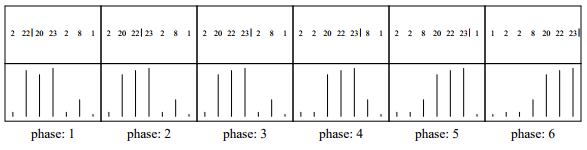
\includegraphics[height=2.5cm,width=13cm]{images/bentleykernighan.png}
\caption{A sequence of stills from an insertion sort algorithm}
\label{fig:bentley-kernighan}	
\end{figure}

Six years later in 1993 Stasko, Badre and Lewis were amongst the first to consider whether algorithm animations assisted learning as much as we might think \cite{StaskoBadreLewis}. Stasko, Badre and Lewis carried out a study which involved attempting to teach two separate groups of students the concept of a ``pairing heap'', with one group using textual descriptions of the algorithm and the other using an animation of the algorithm. Stasko then repeated a similar experiment in 1999 with Byrne and Catrambone. Again, one group used an animation but this time the other group used static diagrams (such as figures from a textbook), instead of textual descriptions like in the previous experiment \cite{StaskoByrneCatrambone}. In both studies the researchers found the results to be disappointing. They found that whilst students in the animation group did perform moderately better than their textual or diagrammatic counterparts, the improvement was not statistically significant.

Despite computer graphic capabilities improving significantly since the 1990s, other more recent studies have shown similar results. The general consensus being that whilst animations do provide a small educational benefit, it is certainly not as large as our intuition would lead us to believe. However, that is not to say that algorithm animations are without use. Stasko, Badre and Lewis suggest that algorithm animations are not particularly effective when students are trying to learn a concept for the first time, but are likely to be much more suitable when students are looking to refine their understanding of a particular notion. The theory is that students should ideally learn the primitive concepts of the algorithm using conventional methods initially, then transition to using animations when looking to clarify and solidify their understanding of certain aspects.

Stasko, Badre and Lewis also reveal a list of guidelines they believe to be effective advice when building algorithm animations, some of which are summarised below:
\begin{itemize}
\item The animation should be augmented with textual descriptions.
\item The animation should include rewind-replay capabilities.
\item Students should be able to build the animation themselves.
\end{itemize}
These guidelines suggest that algorithm animations require accompanying messages that explain the logic of the algorithm at each step. Also, the animation should be interactive in order to engage students in ``active learning'' over ``passive learning''. This interactivity would include intricate controls over the playback of the animation and the ability to modify the input of the algorithm.

\section{Existing Products}
Currently, very few existing tools provide even static illustrations of compilation components (such as syntax trees) and virtually no tools exist that create animations of the compilation process as a whole. There are however, an abundance of web applications that animate more straightforward algorithms, such as sorting or searching algorithms. 

One of the most popular and well implemented is VisuAlgo \cite{visualgo}. VisuAlgo provides an interface for animating various sorting algorithms, including bubble sort, selection sort, etc. As shown in Figure \ref{fig:visualgo}, VisuAlgo implements many of the guidelines we previously listed. It provides impressive playback controls, the ability to choose the input of the algorithm and displays in-depth descriptions of the algorithm's current progress in both plain English and pseudo-code. 

\begin{figure}
	\centering
	\begin{subfigure}[b]{0.45\textwidth}
		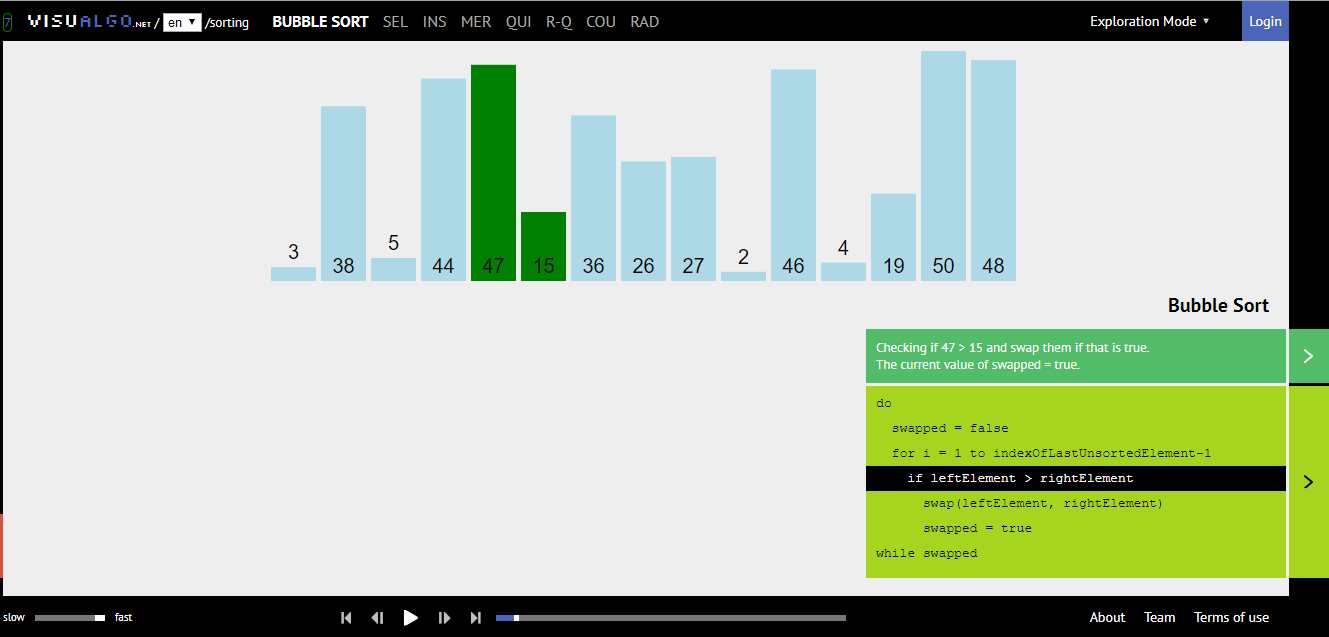
\includegraphics[height=4cm,width=\linewidth]{images/visualgo.png}
		\caption{VisuAlgo}
		\label{fig:visualgo}
	\end{subfigure}
	~
	\begin{subfigure}[b]{0.45\textwidth}
		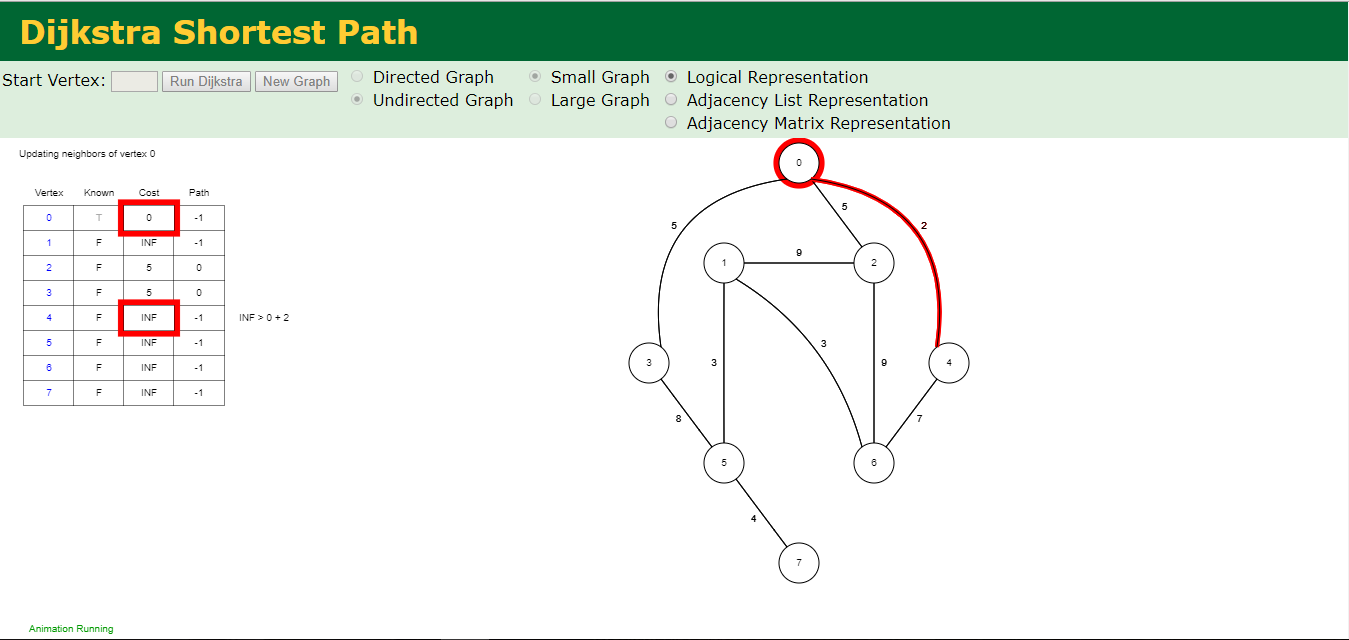
\includegraphics[height=4cm,width=\linewidth]{images/dijkstra.png}
		\caption{The University of San Francisco}
		\label{fig:dijkstra}
	\end{subfigure}
	\caption{Animations of different algorithms from different applications}\label{fig:visualgo-dijkstra}	
\end{figure}


Departing from pure sorting algorithms, the University of San Francisco developed a small web application which animates Dijkstra's algorithm \cite{dijkstra}, as shown in Figure \ref{fig:dijkstra}. Dijkstra's algorithm is arguably more complicated than most sorting algorithms, involving the need to visualise tables and graphs. However, we see that at the expense of this complexity, the application has sacrificed several usability aspects in comparison to VisuAlgo. You cannot define your own input and you cannot pause or rewind the animation. Additionally, whilst some very primitive details are displayed next to the table at each stage, they are far from informative explanations. 

\section{Discussion}
Despite studies showing that algorithm animation is not as effective as we might have initially believed, it would seem that the surprisingly poor performance is due to specific circumstances which could be alleviated if the environment in which an algorithm animation tool was targeted for use was selected more carefully. 

The studies found that algorithm animation was less effective when applied to novice students who were learning the algorithms for the first time, yet could be an effective tool for students who are looking to revise particular concepts. Consequently, any future algorithm animation tool should likely act as a secondary learning resource. Ideally, students should have been taught the concepts using conventional methods to begin with, then the educator can distribute the application to students who can utilise this as a means to refine and clarify understanding.

When considering the previous guidelines proposed by Stasko, Badre and Lewis and how they might affect algorithm animation software, it appears a potential system should:
\begin{itemize}
\item Provide supplementary textual explanations that rationalise and justify the logic of the algorithm.
\item Include rewind-replay functionality that allows the animation to be restarted, or played step-wise, backwards and forwards.
\item Ensure users can create the animation themselves by allowing them to modify the input to the algorithm.
\end{itemize}

% Feel I should remove these last 2 paragraphs but unsure how else to discuss existing products.
After analysing some examples of current products that are available in the area of algorithm animation, such as VisuAlgo and the University of San Francisco's Dijkstra's algorithm animator, it seems there is a trade-off between complexity and usability. In order to animate a considerably more complex algorithm, the University of San Francisco sacrifices much of the visual support and playback control that VisuAlgo is able to provide. 

However, a tool based on compiler animation would need to include both aspects of complexity and usability. The tool would implement an algorithm that is certainly more complex and volatile than even Dijkstra's algorithm, but in order to be educationally effective, it also needs to provide the display of highly input-dependent analytics and implement the usability and interactivity features such as playback control that are embedded within the guidelines of the previous studies.

\chapter{The Fun Programming Language \& Compilation Theory}
This chapter aims to introduce the reader to the main tools and concepts used throughout this dissertation. Firstly, we begin with an small overview of the Fun programming language and its main features. Secondly, we consider how and why compilers parse source code into syntax trees and why some representations of a syntax tree might be more beneficial than others. Thirdly, we take an in-depth look at the three phases of compilation, the latter two of which form the animation basis of this project. Finally, we discuss the use of code templates as a theoretical tool for assisting compiler developers in deciding which object code or assembly language to generate for various constructs within a programming language.

\section{The Fun Programming Language}
Included in Niklaus Wirth's 1975 book {\it Algorithms + Data Structures = Programs}, was a language written entirely in Pascal named ``PL/0''. PL/0 was intended as a small educational programming language, used to teach the concepts of compiler construction. The language contains very primitive constructs and limited operations. Similarly to PL/0, ``Fun'' is a simple imperative language built using ANTLR \cite{antlr}, developed at Glasgow University by David Watt and later extended by Simon Gay. Its purpose is to exhibit various general aspects of programming languages, including the construction of an elementary compiler. The language is provided as a supplementary aid during the delivery of the level 3 computer science course, {\it Programming Languages}, at Glasgow University.

Fun has variables, procedures and functions. Variables can have a declared type of \texttt{int} or \texttt{bool} only. All variables must be initialised with an expression of the same type upon declaration. Procedures have type \texttt{T $\rightarrow$ void} and functions have type \texttt{T $\rightarrow$ T'}. \texttt{T} represents the type of an optional parameter. Procedures return no value (hence \texttt{$\rightarrow$ void}) and functions must return a value of the type \texttt{T'} (hence \texttt{$\rightarrow$ T'}). Fun has one predefined function and one predefined procedure: \texttt{read} and \texttt{write}. \texttt{read()} is a function that returns user input as an integer and \texttt{write(\textbf{int} n)} is a procedure that writes the value of \texttt{n} to standard output. Below is an example Fun program which utilises variables, functions and procedures to calculate and output the factorial value of user input:
\begin{alltt}
\textbf{bool} verbose = true

\textbf{func int} fac (\textbf{int} n):    
    \textbf{int} f = 1   
    \textbf{while} n > 1:    
        f = f*n   
        n = n-1  .   
    \textbf{return} f  
.  

\textbf{proc} main ():  
    \textbf{int} num = read()   
    \textbf{while not} (num == 0):    
        \textbf{if} verbose: write(num) .    
        write(fac(num))    
        num = read() .  
.
 \end{alltt}
 
The Fun programming language has a \textit{\textbf{flat block structure}}. A flat block structure means that variables may reside in either a local or a global scope, and that the same identifier may be declared locally and globally. Since functions and procedures cannot be defined within other functions and procedures, they are always global. A variable that is declared as a parameter of a function/procedure or declared within a function/procedure is considered local. Variables declared outside of any function/procedure are considered global. In the example above, we note that \texttt{verbose} is a global boolean variable, whereas \texttt{n} and \texttt{f} are integer variables local to the function \texttt{fac}. All variables in Fun have a size of 1.

Whilst Fun may differ significantly to other programming languages, particularly in its complexity, it is not the case that the notions it aims to represent are exclusive to the Fun language or the Fun compiler. Fun is sufficiently generic that the core concepts of compiler theory can be delivered in a simple, comprehensible format (due to the simplicity of the language), which then facilitates learners in applying the same logic to more complex constructs in other languages.

\section{Syntax Trees}
During compilation, a source program is parsed into a \textit{\textbf{syntax tree}}. A syntax tree is a hierarchical syntactic representation of a source program; with global statements towards the root, and more deeply nested statements towards the leaves. We typically consider two types of syntax tree: the \textit{\textbf{parse tree}} (sometimes called a concrete syntax tree) and the abstract syntax tree (AST). Translating a source program into a syntax tree means the compiler can more easily reason about the underlying structure and grammatical nature of the program, which is necessary for certain stages of compilation.

A parse tree retains all information about a program, including the information that may appear to be unnecessary, such as white-space and parentheses. Conversely, an AST is a smaller, more concise adaptation of the parse tree. An AST usually ignores redundant details which are derivable from the shape of the tree. Figure \ref{fig:parse-abstract-tree} demonstrates the visual differences between a parse tree and an AST of the same hypothetical Fun program. 

\begin{figure}[h]
	\begin{subfigure}[b]{0.5\textwidth}
		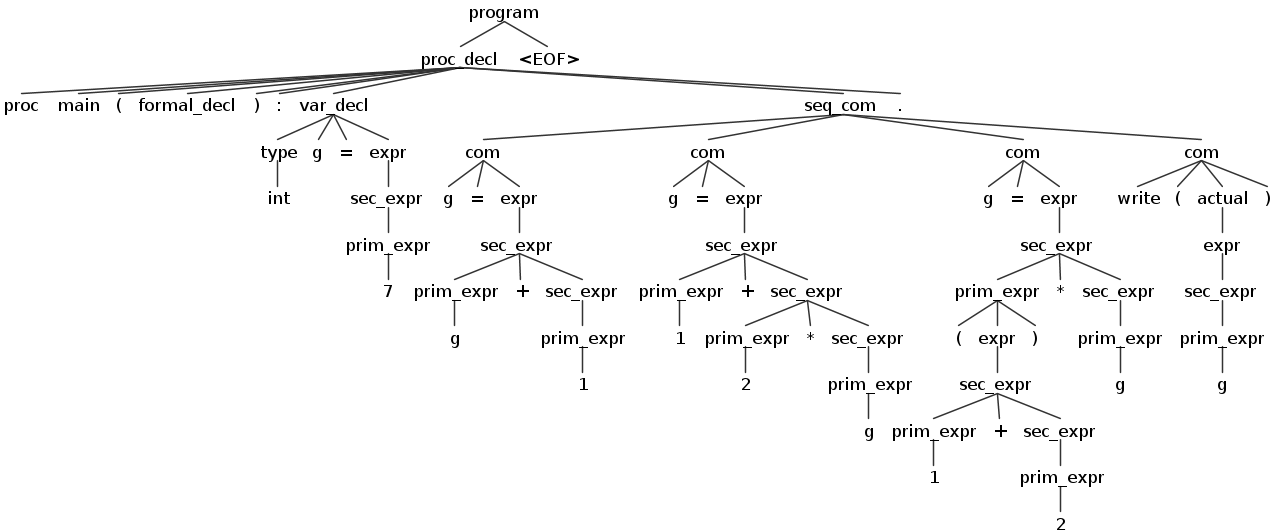
\includegraphics[height=5.5cm,width=\linewidth]{images/2-2a.png}
		\caption{Parse tree}
		\label{fig:ANTLR-parse-tree}
	\end{subfigure}
	\begin{subfigure}[b]{0.5\textwidth}
		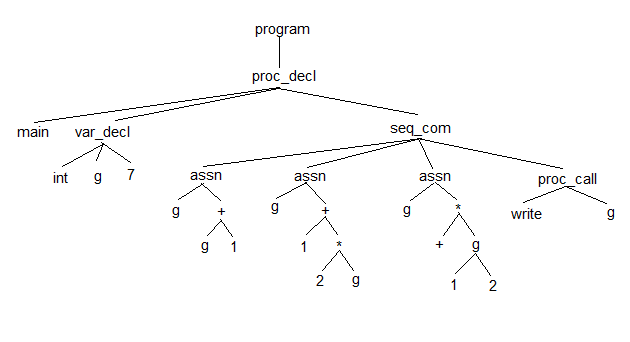
\includegraphics[height=5.5cm,width=\linewidth]{images/2-2b.png}
		\caption{Abstract syntax tree}
		\label{fig:ANTLR-syntax-tree}
	\end{subfigure}
	\caption{Parse tree and AST of the same hypothetical Fun program}\label{fig:parse-abstract-tree}	
\end{figure}

At the initial stages of compilation, the compiler will attempt to translate the input program into either a parse tree or an AST. The generated tree is then traversed during contextual analysis and code generation, which is described in detail in Section 3.3. How the compiler chooses to visit each node in the tree during the traversal is language-dependent, but the semantics are typically very similar to that of a depth-first traversal. 

Since ASTs are usually much smaller and less crowded than their parse tree counterparts, they are often far easier to read and understand. Any information that is lost from the conversion of a parse tree to an AST is usually semantic and does not affect how the syntax tree would be evaluated. Consequently, when trying to illustrate syntax tree concepts to students from an educational perspective, we generally prefer to use visualisations of ASTs over parse trees.

\section{Compilation Phases}
In general, compilation is the process of automatically translating high-level code into low-level code. The most common case is to convert a program whose source code is written in some programming language, into an executable program. This compilation process can usually be decomposed into three distinct phases: 
\begin{enumerate}[label=\alph*)]
\item \textit {Syntactic Analysis}
\item \textit {Contextual Analysis}
\item \textit {Code Generation}
\end{enumerate}
If either syntactic or contextual analysis encounters an error (as determined by the language's specification) during its execution, the phase completes, but the remainder of the compilation process is halted and the errors are reported to the programmer. Note that the following subsections assume the compiler is employing an AST representation of a syntax tree. See Figure \ref{fig:compilation-pipeline} for a diagram of a typical compilation pipeline.

\begin{figure}[h]
\centering
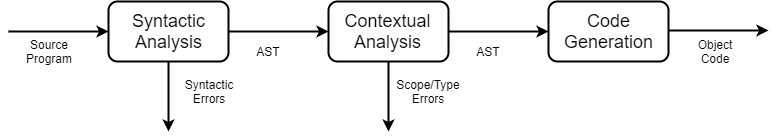
\includegraphics[scale=0.5]{images/3-2a.png}
\caption{Compilation Pipeline}
\label{fig:compilation-pipeline}	
\end{figure}

\subsection{Syntactic Analysis}
Syntactic analysis takes a source program as input and upon success, produces an AST. The purpose of syntactic analysis is to verify whether the source program is well-formed in accordance to the source language's syntax rules. Syntactic analysis can be broken down into \textit{\textbf{lexing}} and \textit{\textbf{parsing}}.

Lexing is the process of breaking down an input program into a stream of \textit{\textbf{tokens}}. A token is simply a single element of the input program. For example, a token could be an individual identifier, operator or keyword. How the compiler chooses to define tokens is dependent upon the implementation of the language. The token stream is then passed as input to the parser. Figure \ref{fig:token-stream} shows how a small excerpt of code may be decomposed into a token stream.

\begin{figure}[h]
\centering
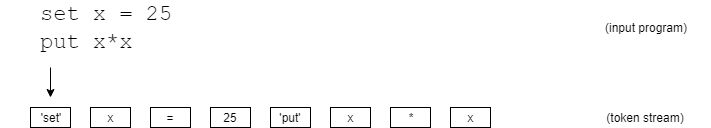
\includegraphics[scale=0.5]{images/token_stream.png}
\caption{Lexing of source code into a token stream}
\label{fig:token-stream}	
\end{figure}

A parser converts a token stream into an AST using some parsing algorithm. The Fun compiler uses \textit{\textbf{recursive-descent}} parsing. Recursive-descent parsing involves ``consuming'' the token stream from left to right. At each token, the parser checks whether the next sequence of tokens are of the correct type, as determined by the language's syntax. The parser carries out this check for every token in the stream. If any checks fail, a syntax error is reported to the programmer. If all tokens are consumed successfully, the parser outputs an AST representing the parsed program.

\subsection{Contextual Analysis}
Upon successful completion of syntactic analysis, the generated AST is traversed  by a contextual analyser. A contextual analyser checks whether the source program represented by the AST conforms to the source language's scope and type rules. Contextual analysis utilises an auxiliary data structure called a \textit{\textbf{type table}} in order to help carry out these checks. Each row of the type table contains three fields of information about a declared variable: its scope (which as discussed in Section 3.1 can be local or global), its identifier and its type. Figure \ref{fig:type-table} demonstrates a small example. The table reveals that the corresponding program contains two integer variables with the identifier \texttt{x} (globally and locally defined) and a global procedure with the identifier \texttt{main} which takes no parameters and returns no value. Contextual analysis can be broken down into \textit{\textbf{scope checking}} and \textit{\textbf{type checking}}.

\begin{figure}[h]
\centering
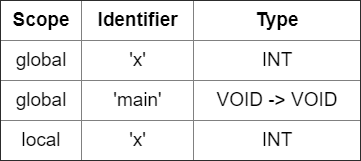
\includegraphics[scale=0.5]{images/type-table.png}
\caption{Type Table}
\label{fig:type-table}	
\end{figure}

Scope checking ensures that every variable used in the program has been previously declared. If the contextual analyser encounters the \textit{declaration} of an identifier as it is traversing over the AST, it inserts the identifier along with its scope and type into the type table. If the contextual analyser finds that there is already an entry in the table with the same scope and identifier, then a scope error is reported to the programmer. Similarly, if the contextual analyser encounters the \textit{usage} of an identifier during the traversal, it checks that the identifier is already in the type table (i.e., has been previously declared). If the identifier cannot be found in the type table, then a scope error is reported to the programmer. Figure \ref{fig:variable-decl-use} shows two ASTs that illustrate the declaration and usage (assignment) of a variable \texttt{n}. The variable \textit{declaration} construct in Figure \ref{fig:variable-decl} would lead the compiler to insert a row into the type table with values: \texttt{[global, n, INT]}. The variable \textit{assignment} construct in Figure \ref{fig:variable-use} would lead the compiler to lookup entries in the type table with identifier \texttt{n} to ensure the variable has been previously declared before attempting to assign a new value to it.

\begin{figure}[h]
	\centering
	\begin{subfigure}[b]{0.3\textwidth}
		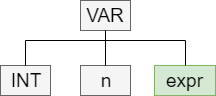
\includegraphics[scale=0.65]{images/variable-decl.png}
		\caption{Variable declaration}
		\label{fig:variable-decl}
	\end{subfigure}
	~
	\begin{subfigure}[b]{0.3\textwidth}
		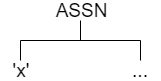
\includegraphics[scale=0.65]{images/variable-use.png}
		\caption{Variable usage}
		\label{fig:variable-use}
	\end{subfigure}
	\caption{ASTs demonstrating the declaration and usage of a variable \texttt{n}}\label{fig:variable-decl-use}	
\end{figure}

Type checking ensures that every operation in the program has operands of the expected type. The rules the contextual analyser uses to determine if an operation has the ``correct'' operands vary from construct to construct. For example, referring back to Figure \ref{fig:variable-use}, we see the construct for variable assignment. In this case, we are assigning the value of some expression, represented by \texttt{expr}, to the variable \texttt{n}. When the contextual analyser encounters this construct during the traversal, it will retrieve the type of \texttt{n} from the type table, then traverse the expression to determine its type. The contextual analyser will then check that the type of the expression is the same as the type of \texttt{n}. For example, given that \texttt{n} was defined as an integer, \texttt{x = 5 + 10} would be a valid assignment, whereas \texttt{x = false} would result in a type error.

\subsection{Code Generation}
Upon successful completion of contextual analysis, the generated AST is traversed by a code generator. A code generator translates the source program into a lower level language, such as assembly language or object code. Code generation utilises an auxiliary data structure called an \textit{\textbf{address table}}. Each entry in the address table contains three fields of information about a declared variable: its scope, its identifier and its address. Figure \ref{fig:address-table} demonstrates a small example. The table reveals how each identifier has been allocated an address in the address space belonging to either local or global variables. Code generation can be broken down into \textit{\textbf{address allocation}} and \textit{\textbf{code selection}}.

\begin{figure}[h]
\centering
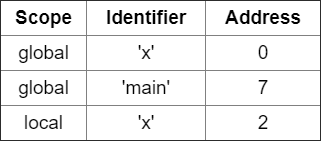
\includegraphics[scale=0.5]{images/address-table.png}
\caption{Address Table}
\label{fig:address-table}	
\end{figure}

Address allocation decides the representation and address of each variable in the source program. If the code generator encounters a variable declaration as it is traversing over the AST, it determines a suitable address and inserts that value along with the corresponding identifier and scope into the address table. In the case of Fun, since all variables have a size of 1, the compiler can simply allocate incrementally consecutive addresses to each variable as it is encountered.

Code selection selects and generates the object code. The developer of the compiler should plan which object code is selected for each construct encountered within the AST. The developer does this by devising a \textit{\textbf{code template}} for each construct in the language.

\section{Code Templates}
When developing a compiler, it is important to consider how each construct in the underlying language should be translated into object code. A code template provides a means of creating a theoretical model for each construct that specifies how the corresponding object code should be selected. Each template is often just a list of directives (written in the plain English) that specifies which assembly language instructions to emit and defines how any constituent expressions/commands of the construct should themselves be considered for translation. 

For example, in Figure \ref{fig:plus} we see an AST that demonstrates the addition of two expressions, where \texttt{expr1} and \texttt{expr2} are sub-expressions of the \texttt{PLUS} construct. Of course, the value of the two expressions must be calculated before attempting to add the two together. In other words, the compiler must evaluate \texttt{expr1} and \texttt{expr2} and emit the object code to load those values into memory \textit{before} emitting the addition object code. Therefore, the code template for the \texttt{PLUS} construct should state that \texttt{expr1} and \texttt{expr2} are to be evaluated before we emit any object code to add the expressions together.

\begin{figure}[h]
	\centering
	\begin{subfigure}[b]{0.3\textwidth}
		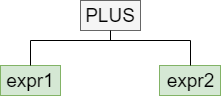
\includegraphics[scale=0.65]{images/plus.png}
	\end{subfigure}
	~
	\begin{subfigure}[b]{0.3\textwidth}
		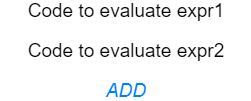
\includegraphics[scale=0.65]{images/plus-template.png}
	\end{subfigure}
	\caption{AST and code template of a \texttt{PLUS} construct}\label{fig:plus}	
\end{figure}

Figure \ref{fig:plus} illustrates the code template as described above. Considering each instruction sequentially, it stipulates that firstly we should generate the object code for \texttt{expr1}, then \texttt{expr2}. Only after emitting both instructions that load the value of these expressions into memory can we emit the \texttt{ADD} object code instruction. 

In the general case, it is often true that the compiler may need to translate some (or all) of the constituent statements of a construct into object code before emitting any object code specific to the original construct itself. Unfortunately, how each construct should be evaluated in regards to code generation is not always immediately clear just from the structure of the AST. This is the scenario in which code templates are practical, as they provide a way to exemplify how each construct in the source language should be translated into object code.

\chapter{Requirements}
This chapter initially discusses the methods via which the requirements of this project, which we will henceforth refer to as the \textit{FunCompiler}, were collected and established. The remainder of the chapter lists the FunCompiler's user stories, functional requirements and non-functional requirements.

\section{Methodology}
The requirements of the FunCompiler were elicited through two main techniques. Firstly, through multiple interviews with Simon Gay. Simon is the current lecturer of the Programming Languages course at Glasgow University. Since both the Fun language and the compilation of Fun programs are delivered during the Programming Languages course, students enrolled in this course will naturally be the target user-base of the FunCompiler. Thus, Simon clearly has the expertise and the experience to offer valuable recommendations on the function and operation of the FunCompiler.

The second technique was to simply utilise the insight gained from performing background research. In particular, we strive to ensure the requirements meet the three guidelines we saw in Section 2.1, proposed by Stasko, Badre and Lewis. Below, the three guidelines have been rephrased to apply directly to the FunCompiler:
\begin{enumerate}[label=Guideline \alph*)]
\item Provide supplementary textual explanations that rationalise and justify the logic of the compiler as it visits each node in the AST.
\item Include rewind-replay functionality that allows the compilation animation to be restarted, or played step-wise, backwards and forwards.
\item Ensure users can create the animation themselves by allowing any arbitrary Fun program as input to the compiler.
\end{enumerate}
\pagebreak
\section{User Stories}
After conducting the interviews and the background research, a set of user stories was devised. User stories are short and simple descriptions of a feature, told from the perspective of a potential user:\\
\begin{table}[h]
\centering
\begin{tabular}{@{}cl@{}}
\toprule
\multicolumn{1}{l}{\textbf{User Story}} & \textbf{Description} \\ \midrule
\textbf{1} & \begin{tabular}[c]{@{}l@{}}As a user, I want to read details of the Fun language, so that I can write \\ valid Fun programs as input and better understand the compilation animations.\end{tabular} \\\\
\textbf{2} & \begin{tabular}[c]{@{}l@{}}As a user, I want to be able to input any Fun program, so that I can learn \\ about the compilation process in the general case, not just for specific examples.\end{tabular} \\\\
\textbf{3} & \begin{tabular}[c]{@{}l@{}}As a user, I want to be able to view the animation of the contextual analysis \\ phase of my program, so that I can understand how the compiler carries out this task.\end{tabular} \\\\
\textbf{4} & \begin{tabular}[c]{@{}l@{}}As a user, I want to be able to view the animation of the code-generation\\ phase of my program, so that I can understand how the compiler carries out this task.\end{tabular} \\\\
\textbf{5} & \begin{tabular}[c]{@{}l@{}}As a user, I want to be able to play different sections of the compilation \\ animation independently (i.e., contextual analysis or code generation), \\ so that I can focus my learning on specific areas.\end{tabular} \\\\
\textbf{6} & \begin{tabular}[c]{@{}l@{}}As a user, I want to be able to see textual descriptions that explain what \\ the compiler is doing at each stage of the animation, so that I can \\ better understand the logic of the compiler.\end{tabular} \\\\
\textbf{7} & \begin{tabular}[c]{@{}l@{}}As a user, I want to be able to see any supplementary information or feedback \\ (including address/type tables, code templates and generated \\ object code), so that I get all the information available in order to help \\ further my understanding.\end{tabular} \\\\
\textbf{8} & \begin{tabular}[c]{@{}l@{}}As a user, I want to be able to replay an animation, so that I can review \\ any details I missed/misunderstood.\end{tabular} \\\\
\textbf{9} & \begin{tabular}[c]{@{}l@{}}As a user, I want to be able to step through the animation at my own \\ pace, so I can more easily understand what is happening during the animation.\end{tabular} \\ \bottomrule \\
\end{tabular}
\end{table}

\section{Functional Requirements}
After creating user stories and using any previous research, a formal list of functional requirements was created. Functional requirements are intended to capture a specific function of a system:

\begin{table}[]
\centering
\begin{tabular}{@{}cl@{}}
\toprule
\multicolumn{1}{l}{\textbf{\begin{tabular}[c]{@{}l@{}}Functional \\ Requirement\end{tabular}}} & \textbf{Description} \\ \midrule
\textbf{1} & Allow users to input any arbitrary Fun program as input to the compiler animator. \\\\
\textbf{2} & Allow users to animate either contextual analysis or code generation separately. \\\\
\textbf{3} & Display the generated AST that represents the input Fun program. \\\\
\textbf{4} & \begin{tabular}[c]{@{}l@{}}Enable a controllable animation over this AST representing one of the two \\ phases (contextual analysis or code generation).\end{tabular} \\\\
\textbf{5} & At each step of the animation, highlight the corresponding node in the AST. \\\\
\textbf{6} & Allow users to play the animation continuously. \\\\
\textbf{7} & Allow users to pause the animation. \\\\
\textbf{8} & Allow users to move forwards through the animation, one step at a time. \\\\
\textbf{9} & Allow users to move backwards through the animation, one step at a time. \\\\
\textbf{10} & \begin{tabular}[c]{@{}l@{}}At each step of the animation, display messages that explain the logic of\\ the compiler, i.e., what it is currently doing, or what it is going to do.\end{tabular} \\\\
\textbf{11} & \begin{tabular}[c]{@{}l@{}}At each step of the animation, display the type table (if contextual analysis) \\ or the address table (if code generation) in its current state during the \\ compilation.\end{tabular} \\\\
\textbf{12} & During code generation, display the code template of each node as it is visited. \\\\
\textbf{13} & \begin{tabular}[c]{@{}l@{}}During code generation, display the emitted object code in its current state during\\ the compilation.\end{tabular} \\\\
\textbf{14} & \begin{tabular}[c]{@{}l@{}}If a user inputs a syntactically invalid Fun program, prevent the animation and\\ report the errors to the user.\end{tabular} \\\\
\textbf{15} & \begin{tabular}[c]{@{}l@{}}If a user inputs a contextually invalid Fun program, allow animation of the\\ contextual analysis phase but disallow animation of the code generation \\ phase and report the errors to the user.\end{tabular} \\\\
\textbf{16} & \begin{tabular}[c]{@{}l@{}}Make the full specification of the Fun language available within the web\\ application.\end{tabular} \\ \bottomrule
\end{tabular}
\end{table}

Along with implementing the core functionality of a compiler animator (along with a few extra features), it is clear to see from functional requirements \textbf{1}, \textbf{6}, \textbf{7}, \textbf{8}, \textbf{9} and \textbf{10}, that we have more than comfortably included the elements necessary to satisfy guidelines a), b) and c).

\section{Non-functional Requirements}
In contrast to functional requirements that detail specific behaviours of a system, non-functional requirements often consider overall utilities of a system, such as security, usability and extensibility:\\
\begin{table}[h]
\centering
\begin{tabular}{@{}cl@{}}
\toprule
\multicolumn{1}{l}{\textbf{\begin{tabular}[c]{@{}l@{}}Non-Functional \\ Requirement\end{tabular}}} & \textbf{Description} \\ \midrule
\textbf{1} & The application must work on all modern browsers. \\\\
\textbf{2} & \begin{tabular}[c]{@{}l@{}}The application must be able to interact efficiently with a Java-based \\ application (the Fun compiler).\end{tabular} \\\\
\textbf{3} & The application must be responsive, at least to a tablet level. \\\\
\textbf{4} & The application must ensure no malicious code can be executed \\ \bottomrule
\end{tabular}
\end{table}

\section{Analysis}
In overview, a typical workflow for the FunCompiler might look as follows: firstly, the user arrives at the website and should be able to view the specification of Fun language before needing to use the animator. Then, the user can type a Fun program into some kind of code editor and choose to animate either contextual analysis or code generation. At this point, if there were any syntactic or contextual errors, they would be reported to the user using the semantics as defined above.

After selecting one of the two phases, the AST that represents the input program is displayed on screen along with playback buttons (play, pause, forwards, backwards). As the animation progresses, nodes within the AST are highlighted to symbolise the current progress of the compiler. As each node is highlighted, detailed information as described above is simultaneously displayed elsewhere on screen. The user is of course free to pause the animation to review the current information displayed, or rewind to review. At any point the user may modify the current input Fun program and select either the same or a different compilation phase, which will halt any current animations.

This potential workflow of the FunCompiler is enough to meet all functional requirements. The non-functional requirements cover issues that are strictly more technical, the solutions to which will be discussed during the system design and the physical implementation.

\chapter{Design}
This chapter covers the aesthetic design process of the FunCompiler. We develop simple low-fidelity wireframe designs of the individual components of the user interface and consider how each of these different components might satisfy our functional requirements. We then look at a more complete design of the user interface and observe how a user might transition from page to page. %Finally, in order to make the website compatible across different screen sizes, we consider a responsive design of the application.

\section{Application Interface}
To act as the first step in realising the project's functional requirements, we develop a series of quick and primitive low-fidelity wireframe designs, each representing an individual component of the user interface. Detailed below are a set of five interface components which when combined satisfy the majority of the application's functional requirements. Each component consists of a wireframe design and considers how the component may meet one or more of the functional requirements (FRs).

\subsection{Code Editor}
The code editor will be the text-area in which users are able to enter code written in the Fun language (FR \textbf{1}). Ideally, the code editor should follow some of the semantics of standard programmatic text editors, including syntax highlighting and auto-indention. Notice that in Figure \ref{fig:code-editor-wireframe} two buttons for ``Contextual Analysis'' and ``Code Generation'' have been attached to the bottom of the code editor. These buttons will trigger the transmission of the input code to the compiler and thus initiate the corresponding animation (FR \textbf{2}).

\begin{figure}[h]
\centering
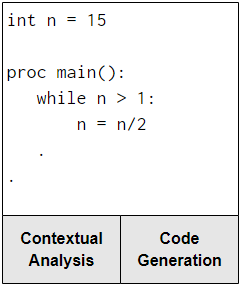
\includegraphics[scale=0.6]{images/code-editor-wireframe.png}
\caption{Code editor wireframe}
\label{fig:code-editor-wireframe}	
\end{figure}

\subsection{AST}
The AST of the input program is the foundation of the animation. The AST will be displayed in a conventional hierarchical tree format where the animator will highlight each node consecutively, corresponding to the progress of the compiler (FR \textbf{3, 5}). For example, along with showing the general structure of the AST for a Fun program, Figures \ref{fig:anim-step-1} to \ref{fig:anim-step-3} demonstrate how the application might animate the AST. At each ``step'' of the animation, the next node in the traversal is highlighted, whilst the previous node is returned to its original state.

\begin{figure}[h]
	\centering
	\begin{subfigure}[b]{0.3\textwidth}
		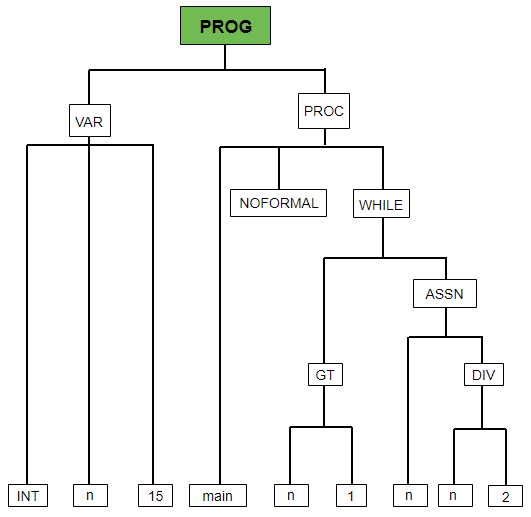
\includegraphics[width=\linewidth]{images/animation-active-wireframe.png}
		\caption{Step 1 of animation}
		\label{fig:anim-step-1}
	\end{subfigure}
	~
	\begin{subfigure}[b]{0.3\textwidth}
		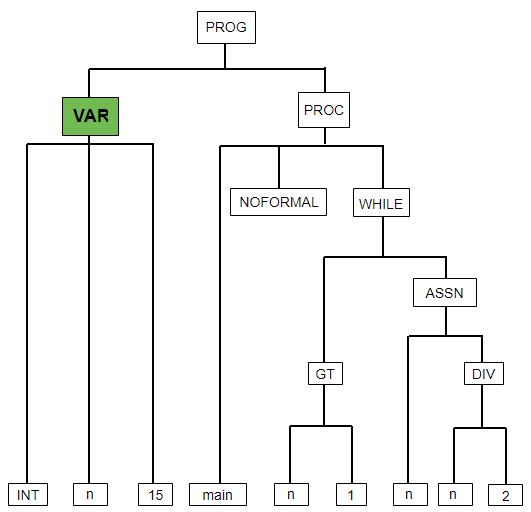
\includegraphics[width=\linewidth]{images/animation-active-wireframe2.png}
		\caption{Step 2 of animation}
		\label{fig:anim-step-2}
	\end{subfigure}	
	~
	\begin{subfigure}[b]{0.3\textwidth}
		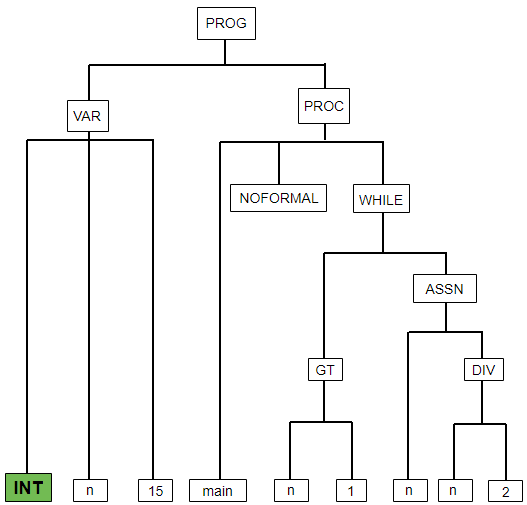
\includegraphics[width=\linewidth]{images/animation-active-wireframe3.png}
		\caption{Step 3 of animation}
		\label{fig:anim-step-3}
	\end{subfigure}	
	\caption{AST wireframes}
	\label{fig:animation-active-wireframe}	
\end{figure}

\subsection{Augmentations}
As the compiler traverses the tree, the application should augment the animation with any supplementary information that may aid the watcher's understanding, including explanatory messages, type/address tables, code templates and object code. We henceforth collectively refer to each of these factors as ``augmentations''. Figure \ref{fig:analytics-ca-wireframe} illustrates the augmentations required for contextual analysis, including a type table and a section to display explanatory messages (FR \textbf{10, 11}). Figure \ref{fig:analytics-cg-wireframe} illustrates similar augmentations for code generation, with the type table replaced by an address table and two added sections to display code templates and object code (FR \textbf{12, 13}). Note that the augmentations, other than the tables, are just textual descriptions/lists, and hence are simply represented as labelled areas in the following wireframes.

\begin{figure}[h]
	\centering
	\begin{subfigure}[b]{0.3\textwidth}
		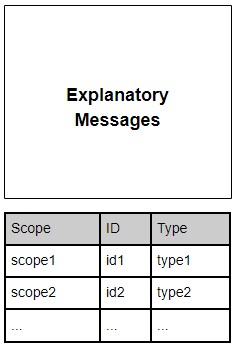
\includegraphics[scale=0.6]{images/analytics-ca-wireframe.png}
		\caption{Contextual analysis augmentations}
		\label{fig:analytics-ca-wireframe}
	\end{subfigure}
	~
	\begin{subfigure}[b]{0.3\textwidth}
		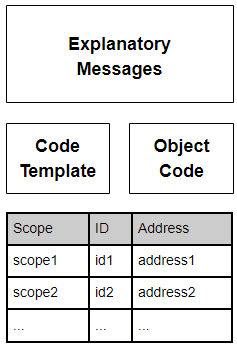
\includegraphics[scale=0.6]{images/analytics-cg-wireframe.png}
		\caption{Code generation \\ augmentations}
		\label{fig:analytics-cg-wireframe}
	\end{subfigure}
	\caption{Augmentations wireframe}\label{fig:augmentations-wireframe}	
\end{figure}

\subsection{Playback Controls}
Users require the ability to play, pause and step through (backwards and forwards) the animation. Figure \ref{fig:playback-wireframe} shows two sets of playback buttons (FR \textbf{4}). Intuitively, when the play button is pressed, it should be replaced with the pause button and vice versa. If the user presses the play button, the animator should highlight the next node in the sequence at regular time intervals (for example, each second) (FR \textbf{6}). If the user presses the pause button, the currently highlighted node should remain highlighted (FR \textbf{7}). If the user presses the forwards/backwards buttons, this will highlight the next/previous node in the sequence, one node per button press (FR \textbf{8, 9}). If the animation is currently playing when a forwards or backwards button is pressed, it should be implicitly paused.

\begin{figure}[h]
	\centering
	\begin{subfigure}[b]{0.3\textwidth}
		
\includegraphics[]{images/playback-play-wireframe.png}
	\end{subfigure}
	~
	\begin{subfigure}[b]{0.3\textwidth}
		
\includegraphics[]{images/playback-pause-wireframe.png}
	\end{subfigure}
	\caption{Playback controls wireframe}\label{fig:playback-wireframe}	
\end{figure}

\subsection{Fun Specification}
 Figure \ref{fig:fun-specification-wireframe}, illustrates the Fun specification broken down into seven sections. Tabs along the top of the component allow the user to navigate between each section. Each section contains varying amounts of information to explain each concept (FR \textbf{16}).
 
 \begin{figure}[h]
\centering
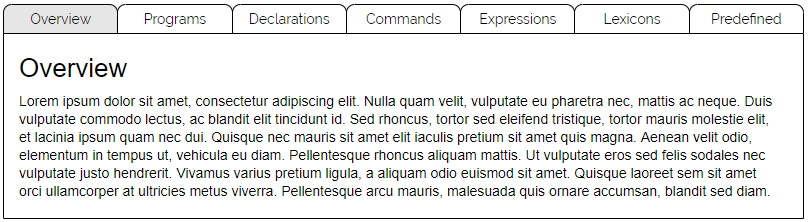
\includegraphics[scale=0.6]{images/specification-wireframe.png}
\caption{Fun specification wireframe}
\label{fig:fun-specification-wireframe}	
\end{figure}

\section{Full Design}
With all necessary components designed, we consider how to combine each of these to create a set of full-sized designs. The presiding design philosophy is that the code editor, the animation and the augmentations are all available within the same view. This is important for two reasons. Firstly, from an educational perspective, there is the obvious necessity that users are able to easily cross-reference between these three components. Secondly, from a usability aspect, as an animation is running, a user should be able to modify the input code and generate a new animation without having the navigate to a different page.

We partition the FunCompiler by splitting the application into three separate pages: the landing page (containing the Fun specification), the contextual analysis animation page and the code generation animation page. We also insert a small navigation bar on each page which includes a link to return to the landing page.

\subsection{Landing Page}
Figure \ref{fig:full1} demonstrates the landing page of the FunCompiler. Here we see that the user has access to the code editor along with access to the full specification of the Fun language. A user can enter a Fun program of their own creation then choose to animate either contextual analysis or code generation by clicking one of the buttons below the code editor. Every page within the FunCompiler has access to the navigation bar seen at the top of the diagram, clicking the ``FunCompiler'' text within this bar will return the user to the landing page.

 \begin{figure}[h]
\centering
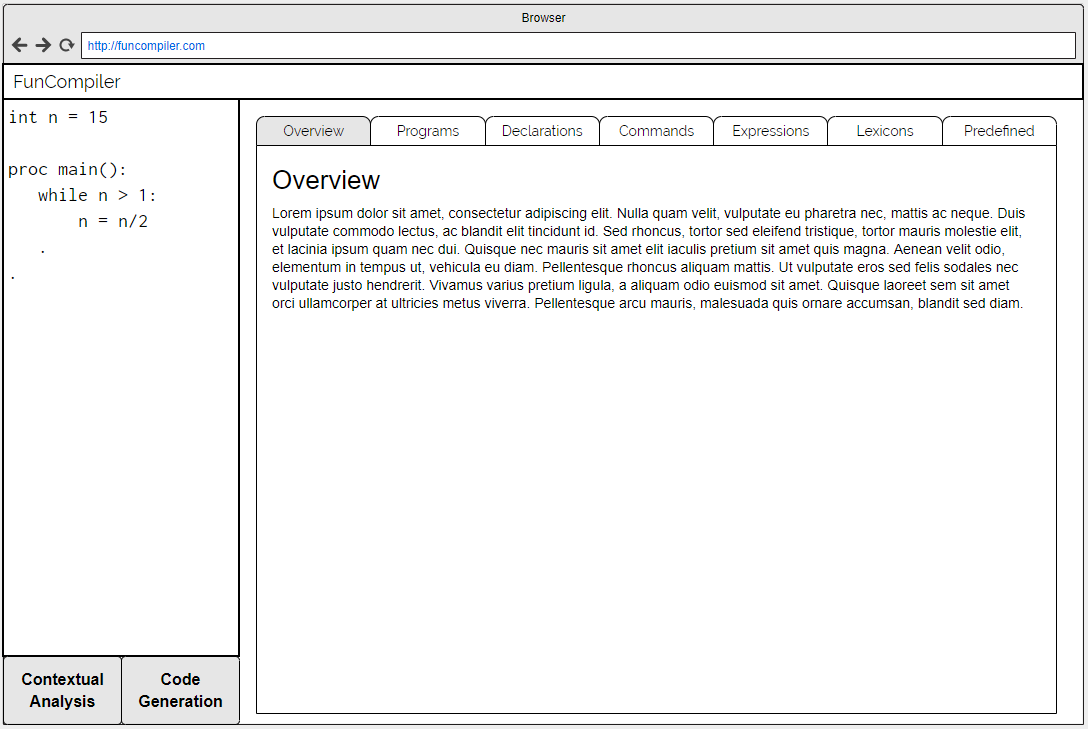
\includegraphics[scale=0.4]{images/full1.png}
\caption{Landing page wireframe}
\label{fig:full1}	
\end{figure}

\subsection{Contextual Analysis Animation Page}
If the user chooses to animate contextual analysis, they are redirected to the page illustrated in Figure \ref{fig:full2}. This page displays an AST generated from the input program, a set of playback controls for the animation, an area to output explanatory messages and a type table. From this page the user still has access to the code editor and is free to modify the input program and generate a new animation. 

 \begin{figure}[h]
\centering
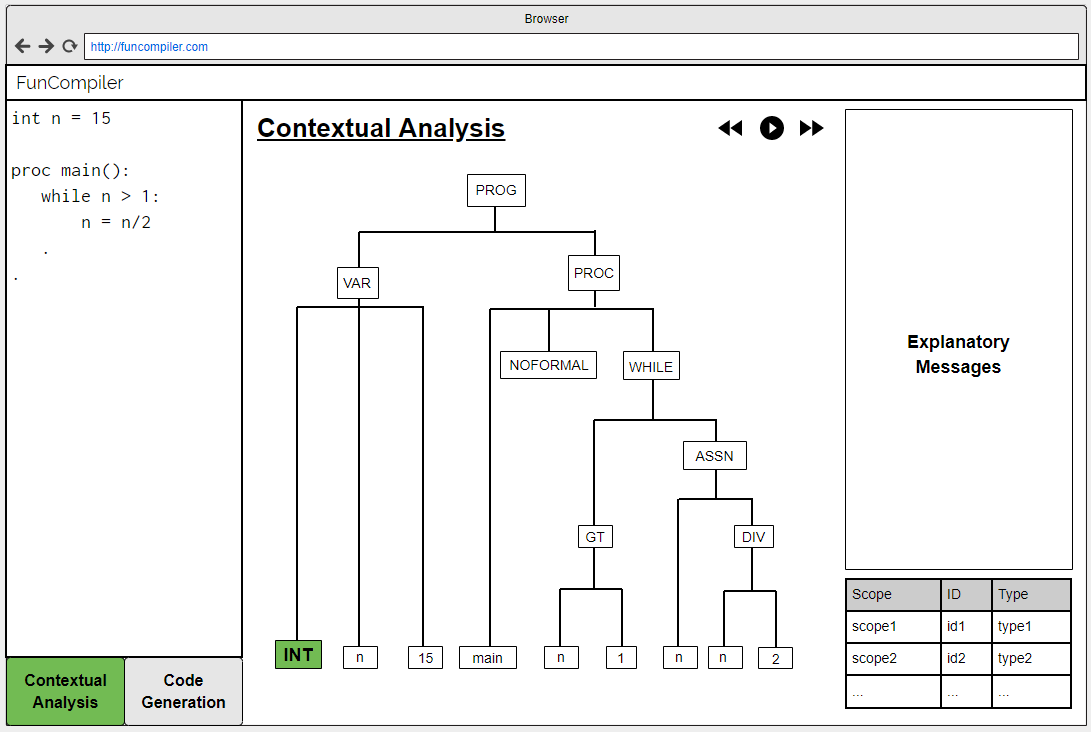
\includegraphics[scale=0.4]{images/full2.png}
\caption{Contextual analysis page wireframe}
\label{fig:full2}	
\end{figure}
\pagebreak
\subsection{Code Generation Animation Page}
If the user chooses to animate code generation, they are redirected to the page illustrated in Figure \ref{fig:full3}. This page displays very similar details to the contextual analysis page, except the type table is swapped for an address table and sections to display code templates and object code have been inserted.

 \begin{figure}[h]
\centering
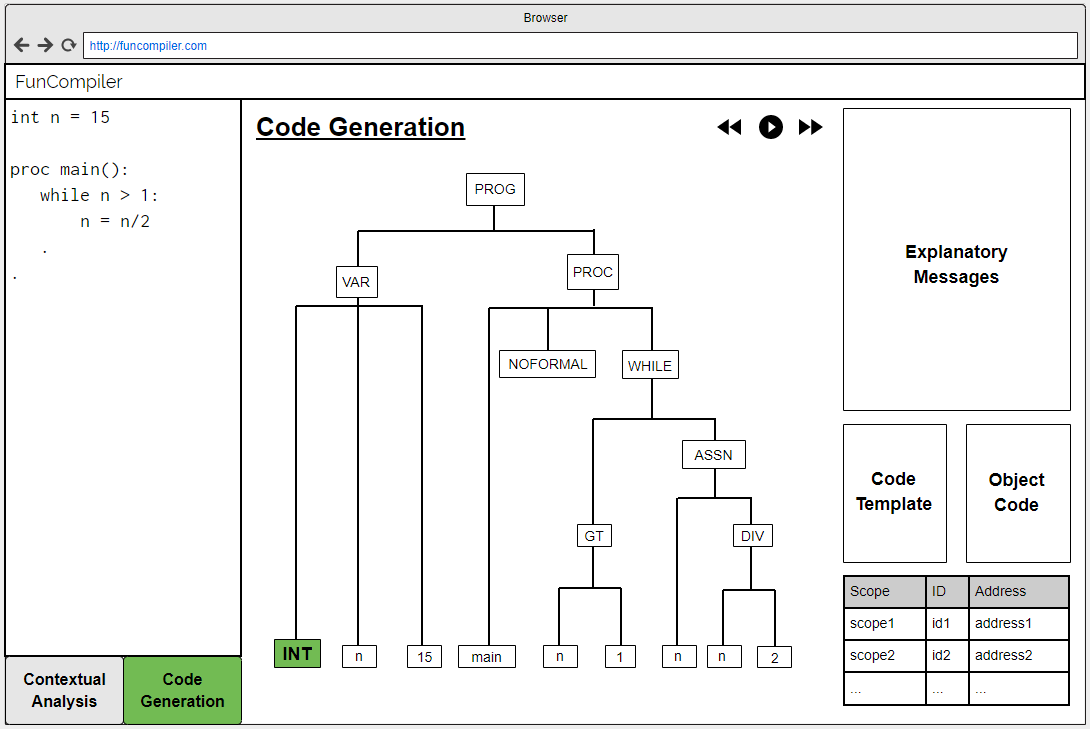
\includegraphics[scale=0.4]{images/full3.png}
\caption{Code generation page wireframe}
\label{fig:full3}	
\end{figure}

\section{Error Handling}
The above component designs successfully covered all but two of the 16 functional requirements. The remaining functional requirements (FR \textbf{14, 15}) are concerned with error handling and preventing certain actions in the event of errors. More specifically, FR \textbf{14} states that we must not allow the animation of either contextual analysis or code generation in that case that the input Fun program contains syntax errors. FR \textbf{15} states that if the input Fun program contains contextual errors, we may animate contextual analysis, but not code generation. In both cases, we present the user with the relevant errors if they try to execute a prohibited action. In order to retain space for the more important aspects of the interface, when a user attempts to submit an invalid program, we simply display the errors as in a pop-up window without disturbing the core contents of the page, as illustrated in Figure \ref{fig:syntax-error-wireframe}. With this final addition in place, we have successfully realised all of the FunCompiler's functional requirements.

 \begin{figure}[h]
\centering
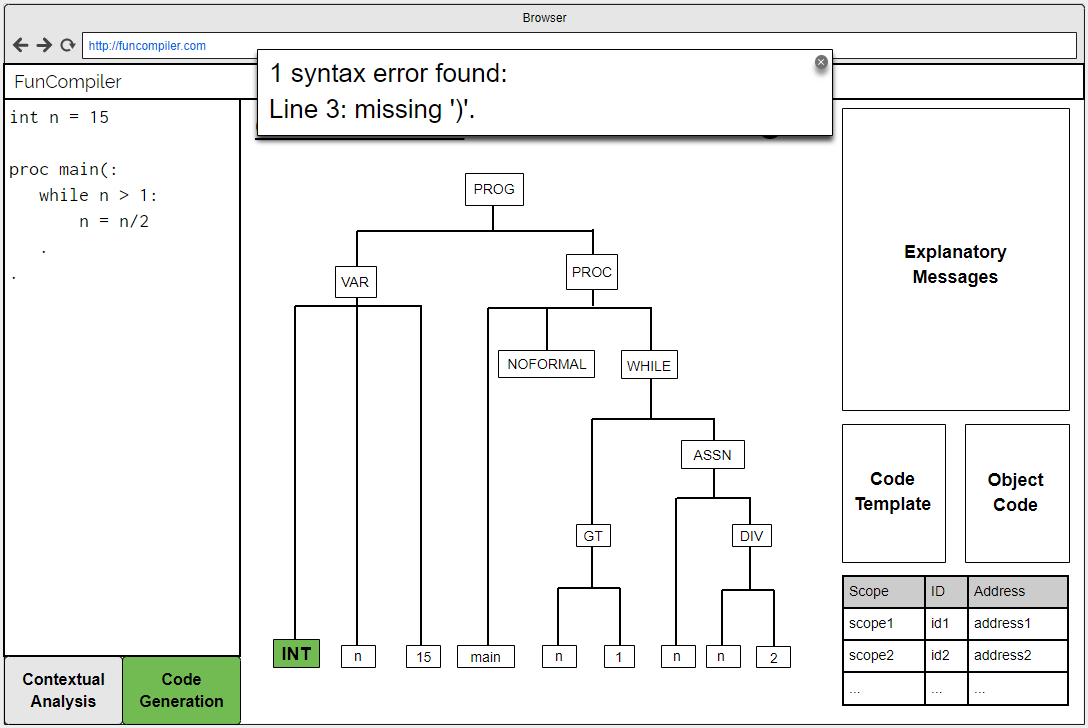
\includegraphics[scale=0.4]{images/syntax-error-wireframe.png}
\caption{Syntax error wireframe}
\label{fig:syntax-error-wireframe}	
\end{figure}


%Put in implementation mayb
%Consequently, it was decided that the FunCompiler would follow the principles of single-page applications (SPAs). SPAs aim to significantly reduce the number of page refreshes websites undergo when the user requests new information or desires to see a different view (i.e., clicks a button). Treating the FunCompiler as an SPA would mean that when users, for example, submit a Fun program, the application will dynamically load the animation into view, without requiring a page refresh. The advantage of SPAs is that for small websites, you can create a much faster workflow which appears seamless. SPAs do have downsides, usually in terms of forcing too much processing on the client when websites grow large, and search engine optimisation. Fortunately, the FunCompiler suffers from neither of these problems.

%\subsection{Fun Specification}
%Since most users of the FunCompiler will be students enrolled in the Programming Languages course at Glasgow University, they will likely already have access to the full specification of the Fun language. However, embedding the Fun specification within the web application is valuable for two reasons. One, it is simply a matter of convenience, students will be able to find all the resources they need in one place. Two, inclusion of the specification helps not preclude the possibility that users could be non-students, as they would not have access to the specification otherwise. 

%%%%%%%%%%%%%%%%
%              %
%  APPENDICES  %
%              %
%%%%%%%%%%%%%%%%
\begin{appendices}

\end{appendices}

%%%%%%%%%%%%%%%%%%%%
%   BIBLIOGRAPHY   %
%%%%%%%%%%%%%%%%%%%%

\bibliographystyle{plain}
\bibliography{bib}

\end{document}
